\chapter{Tratamiento de series temporales de clasificación multivariadas}
En este capítulo se describirán las características principales de las series temporales de clasificación multivariadas, así como diferentes métodos de preprocesamiento que se han utilizado durante el estudio para limpiar dichas series e intentar mejorar los resultados.\newline

Las series temporales multivariadas de clasificación, al igual que cualquier otro conjunto de datos, deben ser preprocesadas para ofrecer un mejor rendimiento a la hora de predecir.\newline

Podemos definir una serie temporal multivariada como $S$, la cual está formada por un conjunto de series temporales univariadas, es decir $S = \{S_1,S_2,...,S_n\}$, cada una de estas series univariadas tienen sus propias características. Las series temporales multivariadas de clasificación son caso de serie temporal multivariada para las cuales además de las series univariadas existen etiquetas en el conjunto de datos. Para las series temporales multivariadas de clasificación existen dos tipos. \newline

El primer tipo de serie temporal multivariada de clasificación es aquella donde cada una de las series temporales univariadas tienen asociadas una clase, es decir $ S = \{(S_1,y_1), (S_2,y_2), ..., (S_n,y_n)\}$, donde cada $S_x$ es una serie univariada e $y_x$ es su clase asociada. Un ejemplo de serie temporal de este tipo puede ser las formadas por imágenes, cada una de las imágenes tiene una clase asociada.\newline

El segundo tipo de serie temporal multivariada es aquella donde en cada momento el conjunto de series univariadas tienen asociada un clase, es decir $S = \{(S_{11},S_{12},...,S_{1m},y_1),(S_{21},S_{22},...,S_{2m},y_2)\}, ..., (S_{n1},S_{n2},...,S_{nm},y_n) $ , donde $S_{xt}$ es el valor asociado a la serie univariada $x$ en un momento $t$ e $y_x$ es la clase asociada a dicho momento. Un ejemplo de este tipo de serie temporal puede ser predecir el movimiento de una persona a partir de los datos obtenidos de diferentes sensores.\newline

A efectos prácticos, esto significa que dependiendo del tipo de series multivariada que sea las series univariadas se encuentran como filas (primer tipo) o como columnas (segundo tipo) y se debe tener en cuenta a la hora de realizar preprocesamiento.\newline

A diferencia del tratamiento normal que se le puede hacer a  un conjunto de datos, aquí se tiene que tener en cuenta que las series temporales multivariadas son un conjunto de series temporales que juntas forman la representación de un problema y hacen que sea capaz de aprender una solución. Una sola serie temporal no es suficiente para poder aprender sobre el problema que se estudie pero sí puede tener características totalmente diferentes al resto de series temporales; por ello, el preprocesamiento se debe hacer de forma individual.\newline

Un paso importante en el preprocesamiento si se están utilizando redes neuronales o cualquier otro modelo que se vea afectado por variaciones en la escala de diferentes características ( o serie temporal en este caso ) es la normalización de valores de las series.\newline

Otro tipo de tratamiento necesario para series temporales es analizar valores perdidos en la serie. Si existen valores perdidos hay dos posibilidades; la primera es eliminar dichos valores perdidos, esta opción no es muy recomendable si la serie tiene muy pocos datos, la otra opción es imputar los valores perdidos. Para imputar dichos valores, se puede utilizar biblioteca específicas para series temporales o utilizar métodos clásicos de imputación, aunque estos no tienen por qué tener en cuenta las particularidades de las series temporales.\newline

Un buen método para imputar datos puede ser realizar un media móvil. La idea es calcular la media de los $x$ momentos anteriores y $x$ momentos siguientes, de esta forma se puede imputar cada dato con un valor cercano al resto de valores. La siguiente imagen muestra un ejemplo de media móvil. A parte de este método, se pueden utilizar métodos clásicos de predicción con series temporales como ARIMA, usando los datos anteriores al dato que se quiere imputar y realizar una predicción del valor de dicho dato con el modelo entrenado; sin embargo esto puede ser bastante costoso si hay bastantes datos perdidos ya que habría que generar un modelo para cada uno de ellos. La figura \ref{fig:51} muestra un ejemplo de serie procesada mediante medias móviles.\newline

\begin{figure}[H]
	\centering
	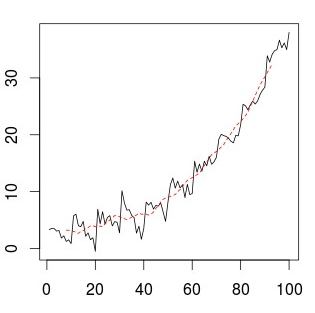
\includegraphics[width=90mm]{imagenes/moving_averages.png}
	\caption{Ejemplo algoritmo medias móviles.}
	\label{fig:51}
\end{figure}

Además de esto, también se pueden analizar los outliers que existan en la serie; si los outliers que se encuentren no aportan ninguna información adicional es mejor modificar su valor. También se podrían eliminar pero esto podría provocar una pérdida de información importante, por ello es mejor no hacerlo.\newline

Para la detección de outliers se puede utilizar cualquier método de detección de outliers univariable. Un método sencillo es el cálculo de outliers mediante IQR ( InterQuartile Range, rango intercuartílico en español ), para ello se calcula el IQR, el $Q_3$ y $Q_1$ el  de los datos para los cuales se quieren detectar outliers; se consideran outliers aquellos datos que estén fuera del rango definido por $[\ Q_1 - f*IQR, Q_3+f*IQR ]\ $ , donde $f$ es una constante.\newline

Normalmente $f$ suele tomar el valor $1.5$ , pero para el caso de las series temporales este valor provoca que se detecten demasiados datos como outliers; por ello, en este estudio se ha utilizado $f=3$ para asegurarse de que los outliers detectados sean realmente anomalías en los datos de la serie y no una pequeña variación. Una vez detectados los outliers, se pueden utilizar diferentes métodos para modificar dichos outliers, por ejemplo el método comentado anteriormente (medias móviles).\newline

Otro proceso que se puede aplicar es crear ventanas de tiempo, es decir, en vez de utilizar solamente los datos en un momento dado, utilizar también los datos de n momentos anteriores para intentar mejorar el rendimiento de un clasificador. Elegir el tamaño de la ventana puede ser complicado ya que la ventana se aplica por igual a todas las series, por lo que requiere de experimentación para comprobar si hay una mejora en el rendimiento. La imagen \ref{fig:52} muestra un ejemplo de uso de ventanas en series temporales.\newline


\begin{figure}[H]
	\centering
	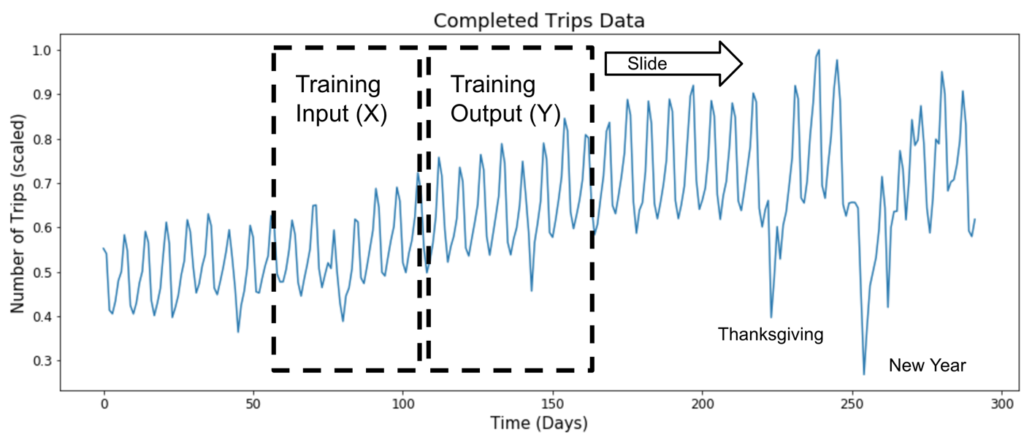
\includegraphics[width=100mm]{imagenes/sliding_window_ts.png}
	\caption{Ejemplo método de la ventana.}
	\label{fig:52}
\end{figure}
\verticalspace

Por último, se puede aplicar una selección de características, o en este caso de series temporales; para ello se pueden utilizar algoritmos de selección de características como por ejemplo Boruta \cite{kursa2010boruta}, este algoritmo utiliza un modelo RandomForest y comprueba qué características son las más utilizadas 
